\documentclass[a4paper]{article}
\usepackage[utf8]{inputenc}
\usepackage[spanish, es-tabla, es-noshorthands]{babel}
\usepackage[table,xcdraw]{xcolor}
\usepackage[a4paper, footnotesep = 1cm, width=20cm, top=2.5cm, height=25cm, textwidth=18cm, textheight=25cm]{geometry}
%\geometry{showframe}

\usepackage{tikz}
\usepackage{amsmath}
\usepackage{amsfonts}
\usepackage{amssymb}
\usepackage{float}
\usepackage{graphicx}
\usepackage{caption}
\usepackage{subcaption}
\usepackage{multicol}
\usepackage{multirow}
\setlength{\doublerulesep}{\arrayrulewidth}
\usepackage{booktabs}
\usepackage{mathrsfs,amsmath}
\usepackage{hyperref}
\hypersetup{
    colorlinks=true,
    linkcolor=blue,
    filecolor=magenta,      
    urlcolor=blue,
    citecolor=blue,    
}

\newcommand{\quotes}[1]{``#1''}
\usepackage{array}
\newcolumntype{C}[1]{>{\centering\let\newline\\\arraybackslash\hspace{0pt}}m{#1}}
\usepackage[american]{circuitikz}
\usetikzlibrary{calc}
\usepackage{fancyhdr}
\usepackage{units} 

\graphicspath{./Imagenes}

\pagestyle{fancy}
\fancyhf{}
\lhead{22.05 ASSD}
\rhead{Mechoulam, Lambertucci, Rodriguez, Londero}
\rfoot{Página \thepage}

\begin{document}

\subsection{Introducción}

En el presente informe se desarrolló un circuito el cual convierte una señal analógica en digital y luego de vuelta a analógica, con tres modos de funcionamiento distintos: frecuencia arbitraria de sampleo, step y free-running.

\begin{figure}[H]
\centering
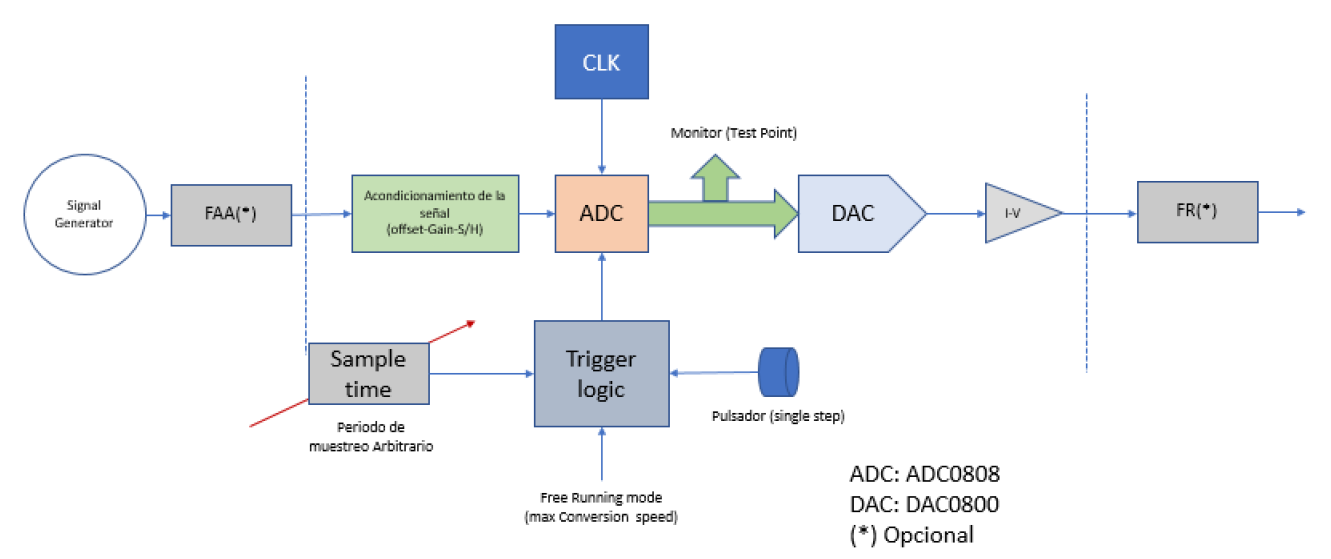
\includegraphics[width=0.9\linewidth]{ImagenesEjercicio1/consigna.png}
\caption{Diagrama en bloques del circuito pedido.}
\label{consigna}
\end{figure}

\subsection{Conversor ADC0808}

El \href{https://www.ti.com/lit/ds/symlink/adc0808-n.pdf}{ADC0808} es un conversor analógico-digital de ocho bits con ocho canales multiplexados y salida binaria paralela. En el presente informe se utilizó un único canal analógico. Este conversor está compuesto por una red en escalera 256R conectada a un árbol de llaves, el cual compara los distintos valores proporcionados por dicha red con la entrada analógica. Es así que, mediante el registro de aproximaciones sucesivas, el cual realiza una búsqueda binaria con todos los valores posibles de la red escalera hasta converger a un valor digital óptimo, el ADC0808 logra realizar la conversión analógica-digital.

\begin{figure}[H]
\centering
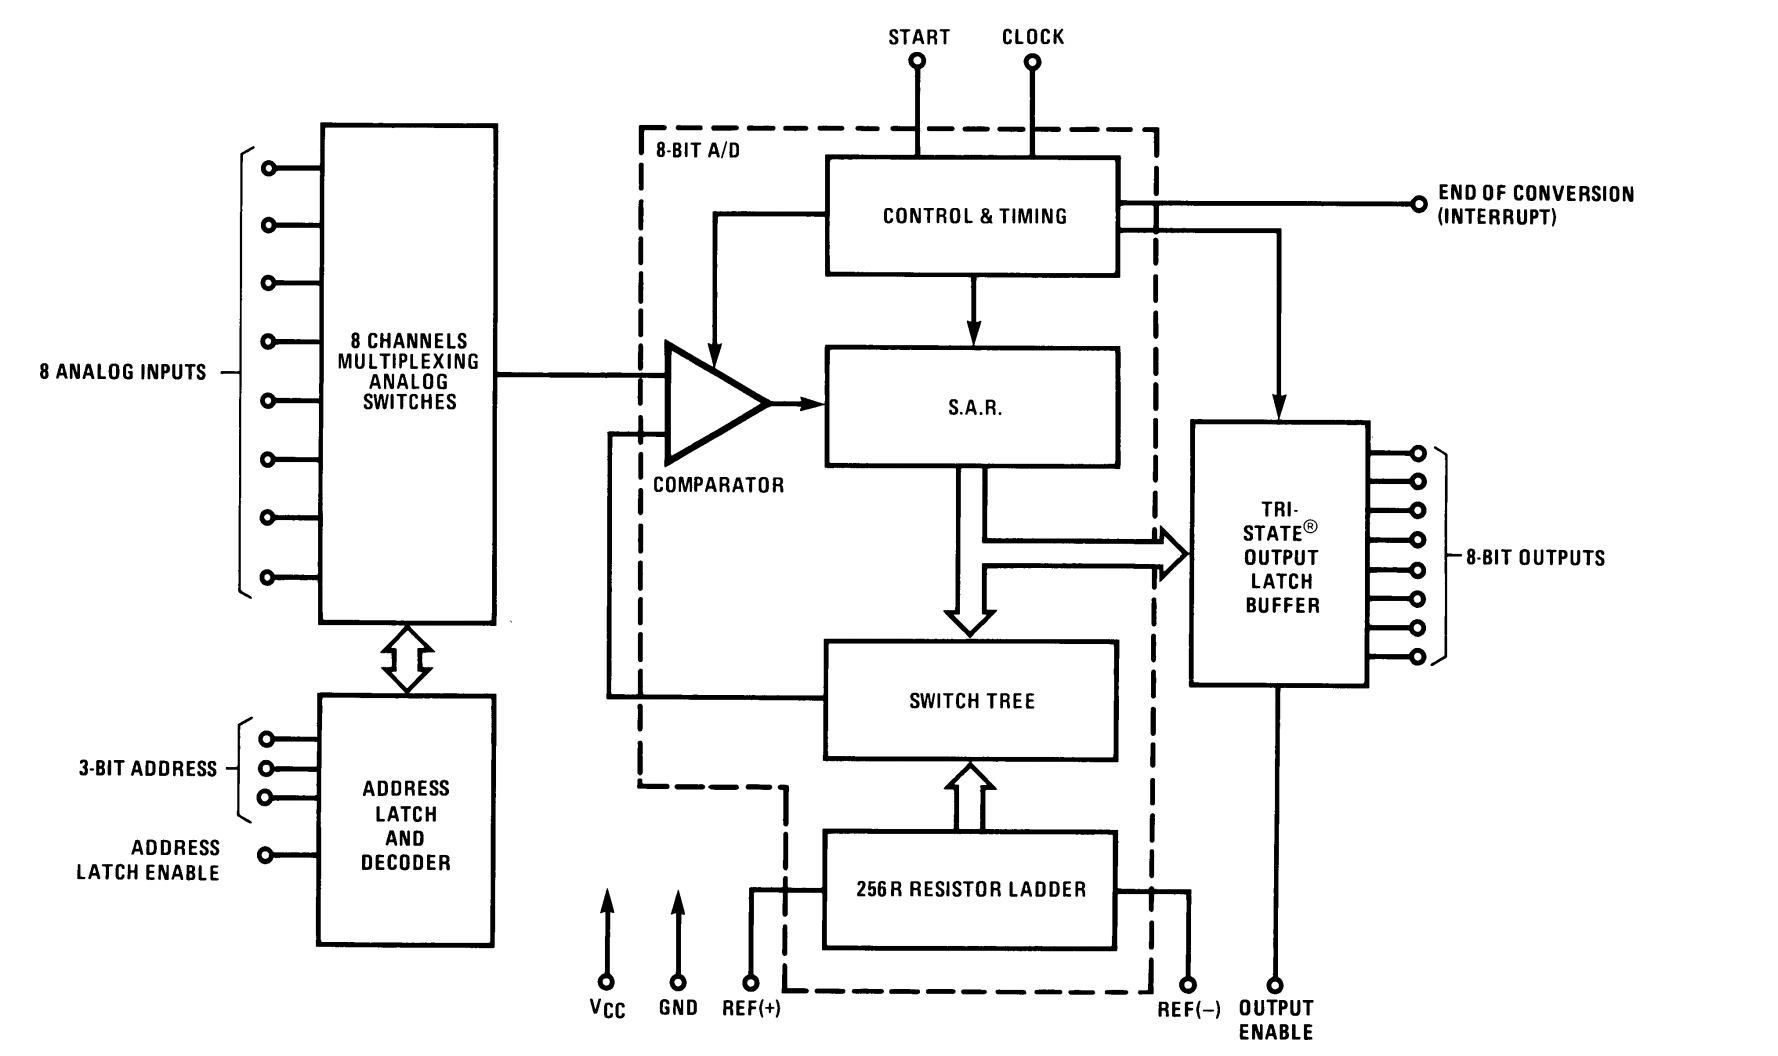
\includegraphics[width=0.75\linewidth]{ImagenesEjercicio1/ADC_BLOCK.png}
\caption{Diagrama en bloques simplificado del conversor ADC0808.}
\label{ADC_BLOCK}
\end{figure}

A continuación, se detalla la funcionalidad de cada pin del integrado mostrado en la Figura (\ref{ADC_BLOCK}) de manera simplificada donde se puede observar el diagrama temporal en la Figura (\ref{ADC_TIMING}).

\begin{itemize}
\item \textbf{8 Analog Inputs}: Aquí se colocan las entradas analógicas que se desean convertir. Se utilizó únicamente una sola de estas entradas, mientras que el resto se las conectó a tierra para evitar el ruido electromagnético.
\item \textbf{3-bit Adress}: Esta entrada binaria permite seleccionar qué entrada analógica se utiliza para realizar la conversión. Estas entradas se conectaron permanentemente a tierra, de manera tal que siempre se realice la conversión con la primer entrada analógica.
\item \textbf{Adress Latch Enable}: Para un valor alto, el ADC0808 mantiene registro del último adress ingresado. Se conectó a VCC.
\item \textbf{VCC}: Tensión positiva de alimentación, se utilizó el valor de $5V$ resultando en una resolución a la salida de $19.6mV$ por bit.
\item \textbf{GND}: Tierra del circuito
\item \textbf{REF(+), REF(-)}: Tensiones de referencia para la red escalera 256R. Se conectó la referencia positiva a VCC y la negativa a GND.
\item \textbf{Clock}: El clock utilizado fue cercano al valor máximo extraído de la datasheet, de $1.2MHz$.
\item \textbf{Start}: Esta señal de control inicia un ciclo de conversión.
\item \textbf{End of Conversion}: Esta señal de interrupción pasa a un estado alto cuando se acaba un ciclo de conversión. Si se conecta esta señal a la señal de \textbf{Start} se logra la máxima frecuencia de conversión para una señal de \textbf{Clock} fija.
\item \textbf{8-bit Outputs}: Salida digital paralela de ocho bits.
\item \textbf{Output Enable}: Permite utilizar la funcionalidad tri-state del buffer de salida. Este pin no fue utilizado y fue fijado en un estado alto.
\end{itemize}

\begin{figure}[H]
\centering
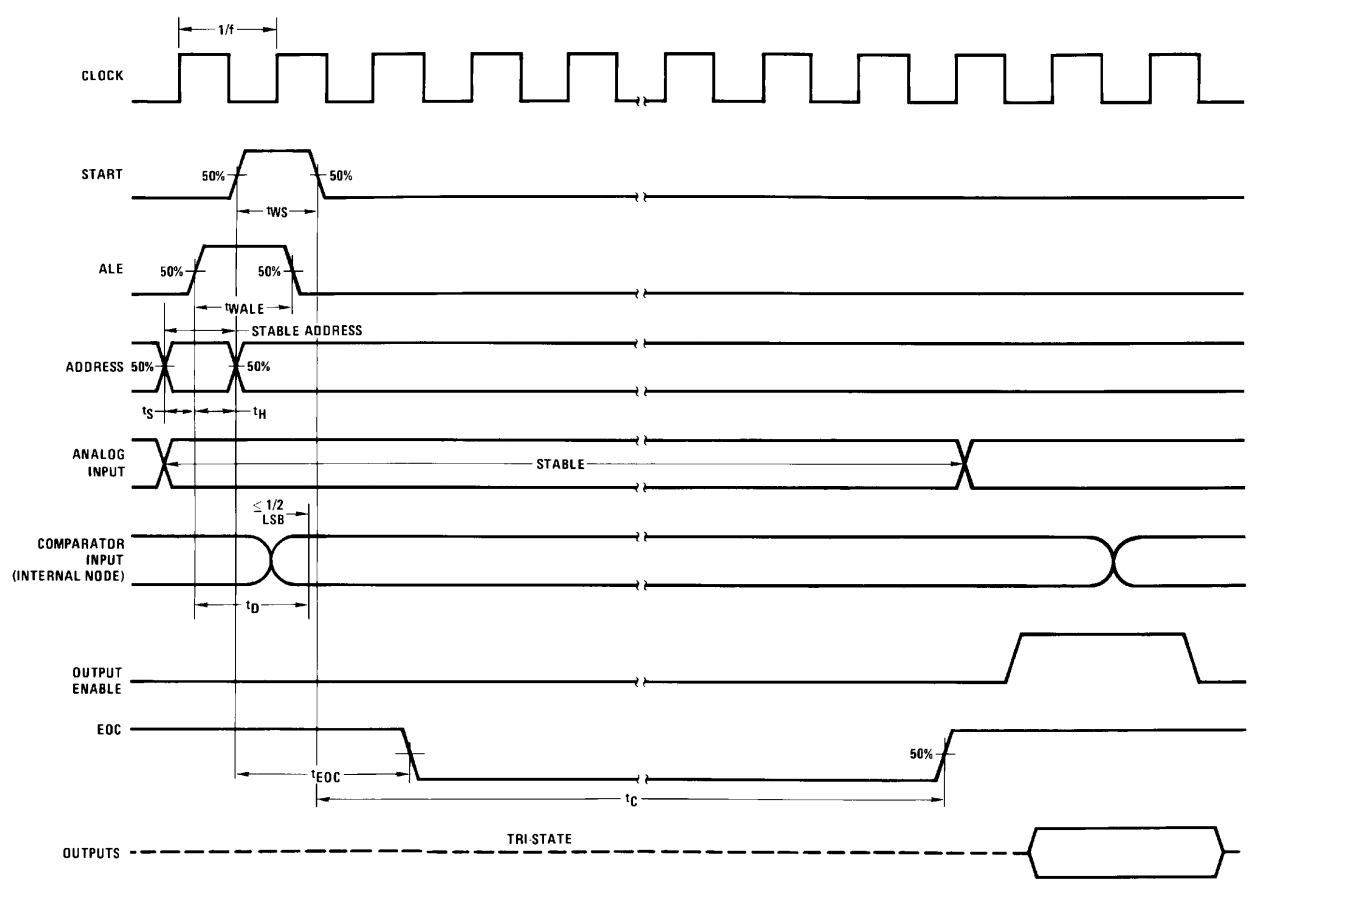
\includegraphics[width=0.9\linewidth]{ImagenesEjercicio1/ADC_TIMING.png}
\caption{Diagrama temporal de las señales de entrada, salida y control del conversor ADC0808.}
\label{ADC_TIMING}
\end{figure}

\subsection{Acondicionamiento de la señal de entrada}

\subsubsection{Offset y enclavamiento}

Dado que la señal que ingresa al ADC0808 debe estar contenida dentro del rango $0V$—$5V$ con un margen de $100mV$, se montó a la señal de entrada sobre un nivel de continua igual a $\frac{5V - 0V}{2} = 2.5V$ para luego limitar con un circuito enclavador a esta resultante entre los rangos permisibles del conversor. El circuito utilizado se detalla en la Figura (\ref{ACOND}).

\begin{figure}[H]
\centering
\includegraphics[width=0.7\linewidth, page = 3]{ImagenesEjercicio1/Components.pdf}
\caption{Circuito de acondicionamiento de la señal de entrada.}
\label{ACOND}
\end{figure}

\subsubsection{Sample \& Hold}

A la hora de realizar el proceso de conversión, el comparador del ADC necesita que la señal de entrada se mantenga estable. Como se verá en la sección siguiente, si no se utiliza un Sample \& Hold, es necesario que la frecuencia de entrada sea lo suficientemente baja como para que el comparador logre hacer su trabajo sin comprometer la precisión de este.

\begin{figure}[H]
\centering
	\includegraphics[width=0.5\linewidth, page = 5]{ImagenesEjercicio1/Components.pdf}
	\caption{Sample \& Hold.}
	\label{fig:sandhold}
\end{figure}

El S\&H seleccionado es el \href{https://pdf1.alldatasheet.es/datasheet-pdf/view/8580/NSC/LF398N.html}{LF398N}. Sabiendo que se posee una taza de conversión máxima de $18.6 \ kHz$, analizado en la sección de restricciones temporales, se tiene que

\begin{equation*}
	T_{acq} = \frac{1}{2\cdot 18.6 \ kHz} \approx 26 \mu s
\end{equation*}

De esta forma, observando el gráfico de la hoja de datos mostrada en la Figura (\ref{chacqtime}) del S\&H, se requiere un capacitor de $10 \ nF$.

\begin{figure}[H]
	\centering
	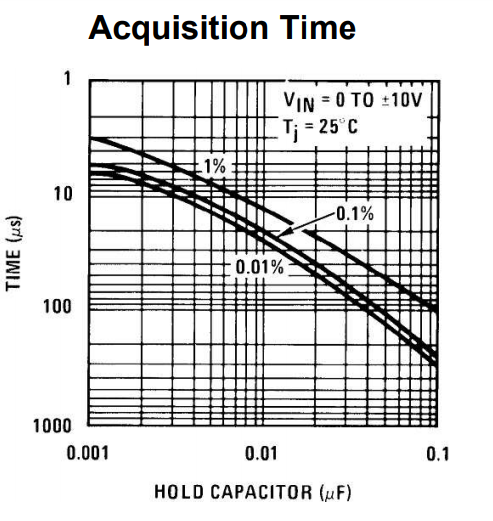
\includegraphics[width=0.4\textwidth]{ImagenesEjercicio1/chacqtime.png}
\caption{Tiempo de adquisición del S\&H en función del capacitor de hold.}
	\label{chacqtime}
\end{figure}

\subsection{Máxima frecuencia de entrada sin Sample \& Hold}

De la datasheet del ADC0808, se tiene que si $V_{CC} = V_{REF+} = 5V$ y $V_{REF-} = 0V$, la resolución será de $19.53125 \frac{mV}{bit}$. Si se utiliza una frecuencia de clock $f_{CLK} = 1.2MHz$ se tiene que $t_{c} = 52\mu s$ con un margen de seguridad como se analizó en la sección de restricciones temporales. Esto implica que la entrada no debe de tener una pendiente mayor a $\frac{19.53125mV}{52\mu s} = 376.6\frac{V}{s}$ para no introducir error en la cuantización de la señal.

Si la señal de entrada se encuentra en el peor caso, es decir, con una excursión de tensión de $-0.1V + V_{REF-}$ a $5V + 0.1V$; esta se encuentra montada sobre un nivel de continua igual a $(5.1V - (-0.1V))/2 = 2.6V$; y esta se puede considerar senoidal gracias a la teoría desarrollada por Fourier; se tiene que la amplitud pico máxima de la senoidal puede ser $2.6V$. Luego, asumiendo el peor caso de la pendiente de la senoidal, para un ángulo igual a cero radianes, lo que permite utilizar la aproximación paraxial, se tiene que

\begin{equation}
\left. \frac{d \left( 2.6V \cdot Sin \left( 2\pi f_{in_{max}} t \right) \right)}{dt} \right|_{t=0} = 2.6V \cdot 2\pi f_{in_{max}} = \frac{19.53125mV}{52\mu s}
\end{equation}

Finalmente, se obtiene que la componente de mayor frecuencia de la señal de entrada para no comprometer la precisión del ACD0808 debe ser como máximo

$$f_{in_{max}} = 23Hz$$

\subsection{Conversor DAC0800}
Se utilizó el integrado \href{https://www.ti.com/lit/ds/symlink/dac0808.pdf?ts=1591879123116&ref_url=https://www.google.com/}{DAC0800}, un conversor D/A de 8 bits con salida diferencial de corriente.
Para convertir esta corriente en un nivel de tensión se utilizó el circuito propuesto por la hoja de datos que se muestra a continuación:
\begin{figure}[H]
	\centering
	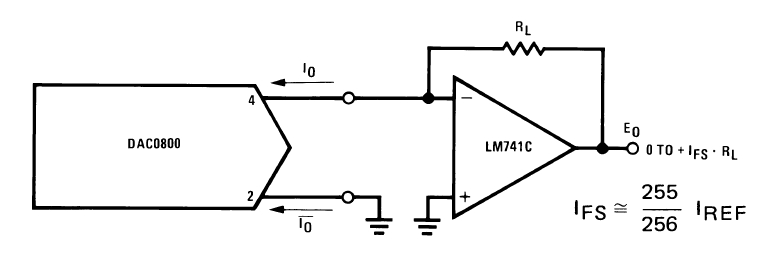
\includegraphics[width=0.7\textwidth]{ImagenesEjercicio1/dacout.png}
\caption{Configuración saldia DAC.}
	\label{fig:dacout}
\end{figure}

La salida va de 0 a $V_{fs}= I_{fs} \cdot R_L$. En cuanto al pinout del DAC es el siguiente:
\begin{figure}[H]
	\centering
	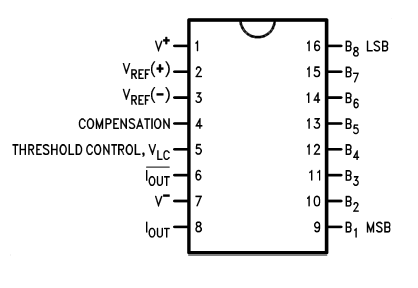
\includegraphics[width=0.5\textwidth]{ImagenesEjercicio1/dacpinout.png}
\caption{Pinout DAC0800.}
	\label{fig:dapinout}
\end{figure}
Donde los pines desde B1 a B8 son las entradas digitales, siendo B1 el bit mas significativo. En cuanto a la salida, es por corriente, y corresponde a los pines 6 y 8, cabe mencionar que dichas corrientes son complementaria, osea su suma da 0. Los pines 2 y 3 son las tensiones $V^+$ y $V^-$ fueron conectadas a 5V y a GND respectivamente, mientras que las tensiones de referencia, si bien dice tensiones, uno debe proveer corrientes de referencia, esto se hace utilizando una resistencia entre vcc y $V_{ref^+}$, al igual que una entre GND y $V_{ref^-}$. En cuanto al pin de threshold fue conectado a masa, mientras que en el pin de comp se conectó un capacitor de 100nF.

\begin{figure}[H]
\centering
\includegraphics[width=\linewidth, page = 2]{ImagenesEjercicio1/Components.pdf}
\caption{DAC y ADC implementados.}
\label{fig:dacydac}
\end{figure}

\subsection{Señal de sincronización de conversión}

\subsubsection{Restricciones temporales}
\vspace{0.2cm}
\textbf{Restricciones teóricas}\\
\\
Si los componentes utilizados tuviesen un tiempo de operación ideal, se podría utilizar un clock tan rápido como se quiera. Sin embargo, esto no sucede. Por parte del integrado ADC0808, se tiene que el tiempo de conversión con una señal de sincronización de $640kHz$ es como máximo $116\mu s$. Luego, el DAC0808 posee un tiempo de estabilización de $100ns$. Por parte del Sample \& Hold utilizado, el LF398N, se tiene que el tiempo de adquisición máximo con un capacitor de hold de $10nF$ es de aproximadamente $26\mu s$ como calculado. Finalmente, se obtienen dos limitantes en tiempo: 

\begin{itemize}
\item El ADC0808 tarda como máximo $116\mu s$ en convertir el valor holdeado de la señal analógica en digital.
\item El LF398N tarda como máximo $26\mu s$ en cargar el capacitor de hold con el valor de la señal analógica en la fase de sampleo.
\end{itemize}

Es por esto, que la rapidez máxima de la señal que gobierna la frecuencia de conversión del circuito es el doble del mínimo entre la inversa de los dos limitantes temporales, es decir, $\frac{1}{2\cdot 116\mu s} = 4.31kHz$.


\vspace{0.3cm}
\textbf{Optimización de la frecuencia de muestreo}\\
\\
Para aumentar aún más las frecuencia de conversión del circuito, se puede generar una señal de control cuyo duty cycle no sea del $50\%$, debido a que mientras el ADC se encuentra convirtiendo, el S\&H no posee ninguna restricción temporal más que la de fuga del capacitor, mientras que si el S\&H está sampleando la señal, el ADC no posee ninguna restricción temporal.

%aca poner grafico de un clock con duty cycle no simetrico donde en la parte que dura poco se esta haciendo el sampleo y en la parte larga se esta haciendo la conversión

Basta con que el duty cycle sea tal que el tiempo de holdeo sea igual al tiempo de conversión del ADC y el tiempo de sampleo se igual al tiempo máximo que tarda el S\&H en cargar su capacitor de hold. Se tiene entonces que

\begin{equation}
DT_{optimo} = \frac{20\mu s}{116\mu s}\cdot 100 = 17.24\% 
\end{equation}
para simplificar el circuito, se tomó $DT = 25\%$, por lo que se tiene que el tiempo de sampleo es de

\begin{equation}
T_{sample} = 0.25 \cdot 116\mu s = 29\mu s 
\end{equation}

Es así que se obtiene una máxima frecuencia de sampleo teórica con las consideraciones de 
$$\frac{1}{116\mu s + 29\mu s} = 6.896kHz$$
\\
\textbf{Aproximación a la máxima frecuencia de muestreo real}\\
\\
Como último paso, se obtuvo una aproximación empírica a la máxima frecuencia de muestreo posible, simulando el integrado ADC0808 con una sola entrada analógica, una frecuencia de clock de $1.28MHz$ y los pines de start y end of conversion cortocircuitados, lo que provee el menor tiempo de conversión posible, obteniendo $50.48\mu s$. Esto no resulta sorprendente, dado que un documento de Texas Instruments acerca del uso del ADC0808 afirma que con una sola entrada analógica se tiene un tiempo de conversión de alrededor de los $50\mu s$.
Finalmente, se tomará una máxima frecuencia de muestreo teórica de $\frac{1}{52\mu s + 26\mu s} = 12.82kHz$, reservándose un margen de seguridad en el tiempo de conversión. Luego, se tiene que el duty cycle será de $\frac{26\mu s}{52\mu}\cdot 100 = 25\%$.

\subsubsection{Circuito generador de la señal de sincronización}

Se partió de un generador de onda cuadrada de $1.28 MHz$, detallado en la próxima sección, el cual será la señal de clock del ADC0808. A esta señal, se la deberá dividir por $\frac{1.28MHz}{12.82kHz} = 99.84$ veces para obtener una señal cercana a la frecuencia máxima de muestreo. Sin embargo, para simplificar la división de frecuencia, se dividirá por $96$ veces y se utilizará un clock de $1.2Mhz$, obteniendo una nueva máxima frecuencia de muestreo de $12.5kHz$.

La división de frecuencia se efectuó de la siguiente manera: la señal de $1.2Mhz$ pasará por un divisor de frecuencia que divide por $48$ veces. Luego, esta señal ingresa a un divisor de frecuencia que divide por dos. Se detalla en la Figura (\ref{DT}) esta operación. Seguido a esto, se realiza la operación AND entre la señal antes de pasar por el divisor, y la señal a la salida del divisor. Así se obtiene una señal de $DT$ del $25\%$.

\begin{figure}[H]
\centering
\includegraphics[width=0.7\linewidth, page = 2]{ImagenesEjercicio1/Graficos.pdf}
\caption{Diagrama temporal de las señales de control del circuito.}
\label{DT}
\end{figure}

Esta señal de frecuencia $f_{conv}$ y duty cycle del $25\%$ posterior a la operación AND es la que se utilizará como señal de control del S\&H. Finalmente, se quiere enviar un pulso de una duración de al menos $t_{ws} = 200ns$ al pin de start del ADC0808 cuando el S\&H comience a holdear, por lo que se utilizará un negador seguido de un detector de flancos para generar esta señal de start. El resultado se detalla en la Figura (\ref{START})

\begin{figure}[H]
\centering
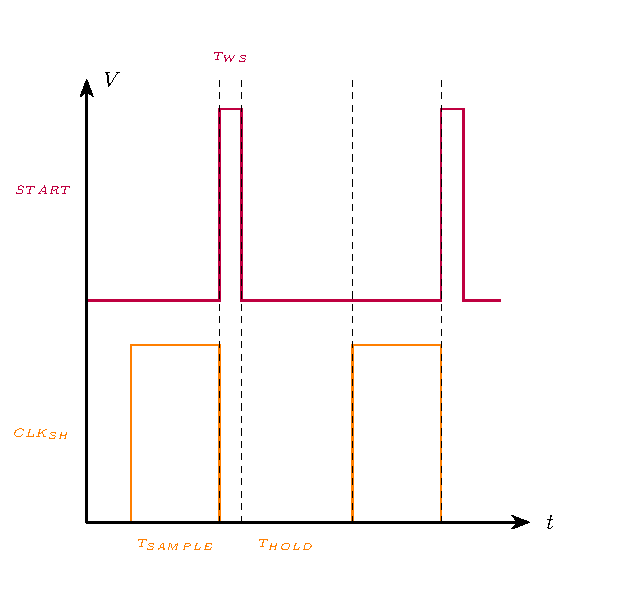
\includegraphics[width=0.6\linewidth]{ImagenesEjercicio1/Graficos.pdf}
\caption{Diagrama temporal de las señales de control del circuito.}
\label{START}
\end{figure}

Así se obtienen todas las señales de control del circuito de una misma señal de clock original, de tal manera que todas estén sincronizadas entre sí. Si se desea disminuir la frecuencia de conversión basta con disminuir la frecuencia $f_{CLK}$ del circuito oscilador presentado a continuación.

\subsubsection{Circuito oscilador}

Se utilizó el circuito mostrado en la Figura (\ref{555}) para generar la señal de clock de $1.2MHz$ la cual no solo será ingresada al ADC0808 sino de la cual se generarán las señales de sincronización del S\&H y de start del conversor.

\begin{figure}[H]
\centering
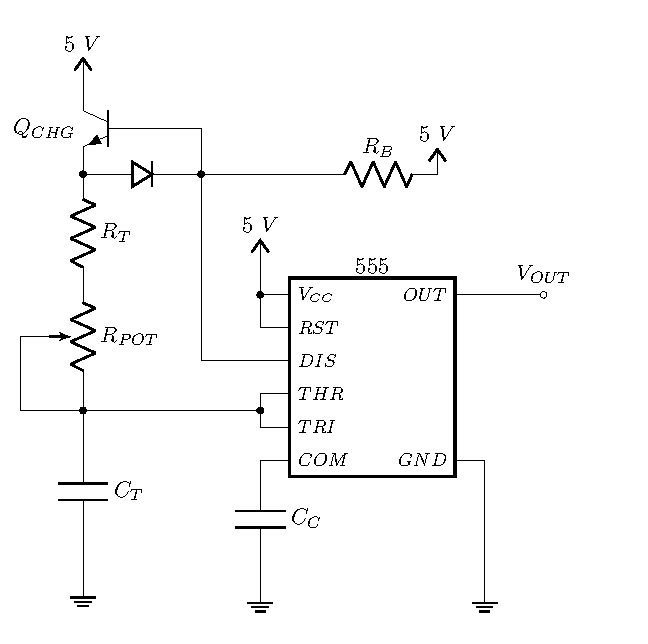
\includegraphics[width=0.6\linewidth, page=1]{ImagenesEjercicio1/Components.pdf}
\caption{Circuito oscilador.}
\label{555}
\end{figure}

Utilizando $R_{T} = 370\Omega$, $R_{POT} = 10k\Omega$ y $C_{T} = 1nF$ se logra obtener

\[ 48.7kHz < f_{CLK} < 1.2MHz\]
por lo que la frecuencia de conversión del circuito total será de

\[ 507Hz < f_{CONV} < 12.5kHz \]

\subsection{FAA y FR}


Tanto para el filtro anti alias como el filtro recuperador se tomaron las mismas especificaciones.
Tomando como $f_p= 5kHz$ que es levemente menor a $\frac{12.5kHz}{2}\approx 6.25kHz $ y una $f_s$= 5.75kHZ.
Se optó por utilizar la aproximación de Legendre debido a la planitud en banda pasante y la gran pendiente que este presenta comparada con la de un Butterworth, obteniendo para una $A_p$=1dB y $A_s$=35dB se obtiene un filtro de orden 14.
\begin{figure}[H]
\centering
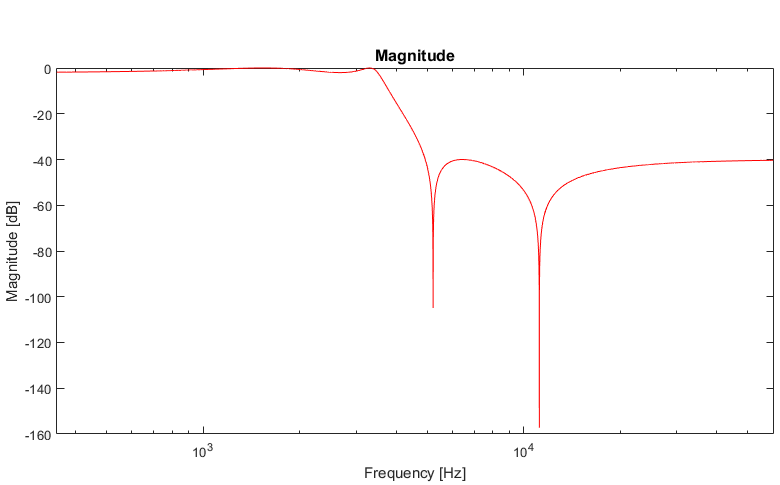
\includegraphics[width=0.7\linewidth, page=1]{ImagenesEjercicio1/magnitude.png}

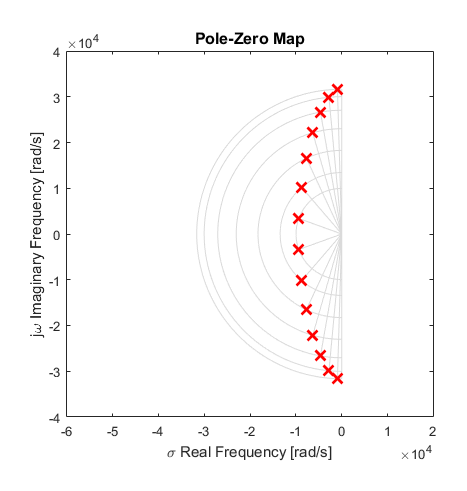
\includegraphics[width=0.5\linewidth, page=1]{ImagenesEjercicio1/pz.png}
\caption{Filtro implementado.}
\label{filtros}
\end{figure}

Las celdas utilizadas para implementar dicho filtro corresponde a la topología Sallen-Key pasa bajos:
\begin{figure}[H]
\centering
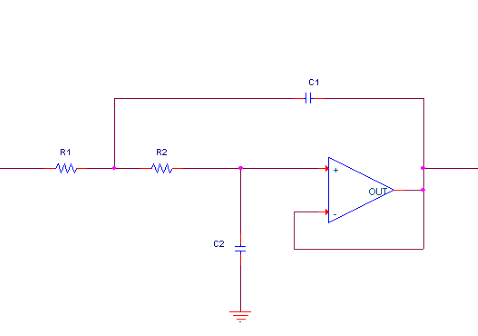
\includegraphics[width=0.8\linewidth, page=1]{ImagenesEjercicio1/SK_LP.png}
\caption{Filtro implementado.}
\label{filtros}
\end{figure}
Si se tuviese que implementar la placa, no se utilizarían filtros implementados de manera discreta sino uno integrado como el MAX291, que es un filtro pasa bajos de Butterworth de orden 8, implementado con switch capacitors, pero debido a que no se pudo encontrar un modelo apto para el proteus, para la simulación se optó por el filtro implementado de manera discreta.
\subsection{Resultados}

Se observan distintas señales características del circuito en la Figura (\ref{result1}), donde la señal amarilla se mide a la salida del filtro anti-alias, la señal azul a la salida del S\&H, la señal roja a la salida del DAC y finalmente la señal verde a la salida del filtro recuperador.

\begin{figure}[H]
\centering
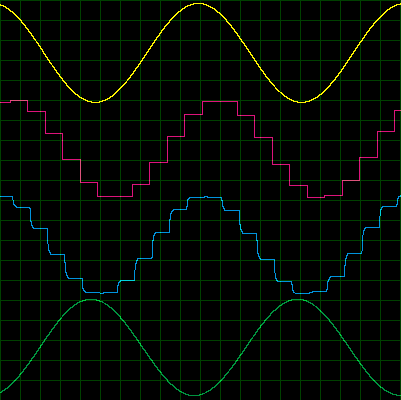
\includegraphics[width=0.5\linewidth, page=1]{ImagenesEjercicio1/result1.png}
\caption{Señales características del circuito.}
\label{result1}
\end{figure}

Se puede ver en la Figura (\ref{result2}) una pérdida de amplitud de más del $10\%$ debido al muestreo.

\begin{figure}[H]
\centering
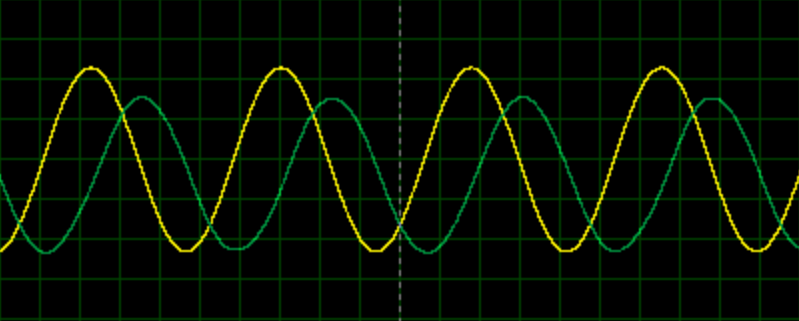
\includegraphics[width=0.8\linewidth, page=1]{ImagenesEjercicio1/result2.png}
\caption{Comparación entre la señal a la salida del filtro anti-alias y el filtro recuperador.}
\label{result2}
\end{figure}

En la Figura (\ref{sh}) se puede ver que los calculos realizados para la señal de control del S\&H fueron correctas.

\begin{figure}[H]
\centering
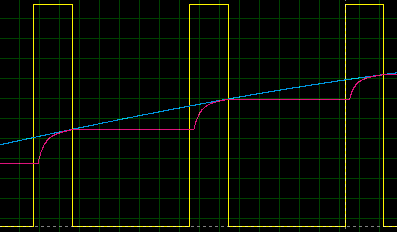
\includegraphics[width=0.8\linewidth, page=1]{ImagenesEjercicio1/S_H.png}
\caption{Señal de control del S\&H, señal de entrada y señal a la salida del S\&H.}
\label{sh}
\end{figure}

\subsection{Mediciones}
Finalmente para comprobar el correcto funcionamiento del circuito se utilizó la máxima $f_{clk}$ admisible por el circuito, de $1.2MHz$, una señal rampa de frecuencia $45Hz$ y una amplitud de $0V$ a $5V$, de tal manera que la pendiente no sea mayor que $376.6\frac{V}{s}$, calculado en la sección de funcionamiento sin S\&H. Si bien el límite teórico sería de aproximadamente $75Hz$ para la frecuencia de la rampa, se eligió esa frecuencia particular debido a que se tenia que el tiempo de conversión real era de $84.5\mu s$ y una resolución real de $19.5 mV$, por lo que si se quiere que en cada muestreo el ADC incremente su salida estrictamente por un solo bit, se deberá de tener una rampa con una pendiente de aproximadamente $\frac{19.5mV}{85.8\mu s} = 227.27 \frac{V}{s}$, por lo que la frecuencia debe ser cercana a $\left(\frac{5V}{227.27\frac{V}{s}}\right)^{-1} = 45.45Hz$.

\begin{figure}[H]
\centering
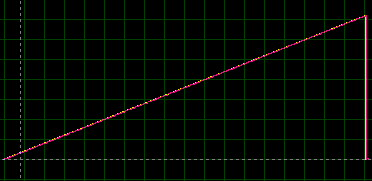
\includegraphics[width=0.8\linewidth]{ImagenesEjercicio1/rampa1.png}
\caption{Rampa a la salida del FAA y a la salida del DAC.}
\label{med1}
\end{figure}

\begin{figure}[H]
\centering
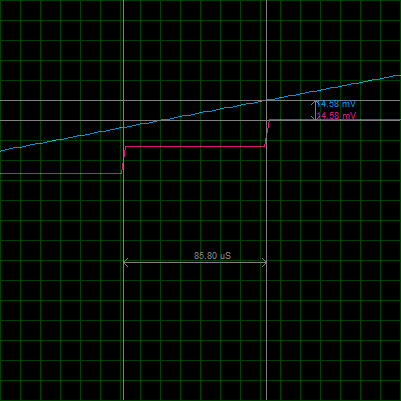
\includegraphics[width=0.8\linewidth]{ImagenesEjercicio1/rampa1zoom.png}
\caption{Medición de la frecuencia de muestreo experimental.}
\label{med2}
\end{figure}
Según los cálculos teóricos realizados en secciones anteriores, se tendrá una frecuencia de muestreo de $\frac{1.2MHz \cdot 2}{96 \cdot 2} = 12.5kHz$. Se midió esta frecuencia de muestreo experimentalmente la cual fue de $11.655kHz$ mostrado en la Figura (\ref{med2}).


\begin{center}
	\LARGE{\textcolor{red}{\textbf{Luego, se se midió el error de cuantización empleando el método de..}}}
\end{center}

Por otro lado, se midió la forma de onda a la salida del DAC a medida que se eliminaban bits menos significativos. Se puede ver el resultado detallado en las siguientes Figuras:

\newpage

\begin{multicols}{2}
\begin{figure}[H]
\centering
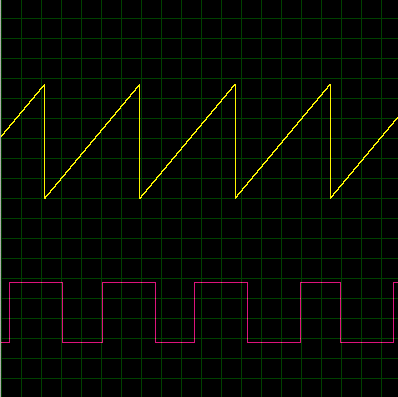
\includegraphics[width=0.5\linewidth]{ImagenesEjercicio1/bit1.png}
\caption{1111 1110}
\end{figure}
\begin{figure}[H]
\centering
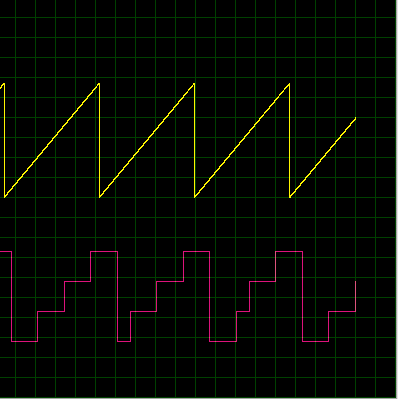
\includegraphics[width=0.5\linewidth]{ImagenesEjercicio1/bit2.png}
\caption{1111 1100}
\end{figure}
\begin{figure}[H]
\centering
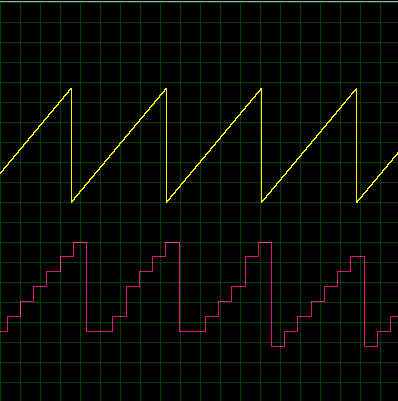
\includegraphics[width=0.5\linewidth]{ImagenesEjercicio1/bit3.png}
\caption{1111 1000}
\end{figure}
\begin{figure}[H]
\centering
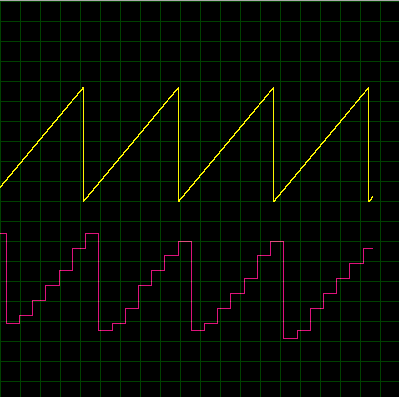
\includegraphics[width=0.5\linewidth]{ImagenesEjercicio1/bit4.png}
\caption{1111 0000}
\end{figure}
\begin{figure}[H]
\centering
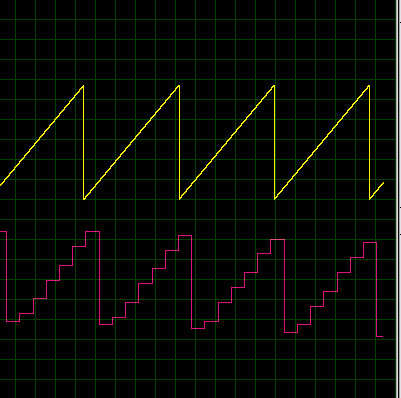
\includegraphics[width=0.5\linewidth]{ImagenesEjercicio1/bit5.png}
\caption{1110 0000}
\end{figure}
\begin{figure}[H]
\centering
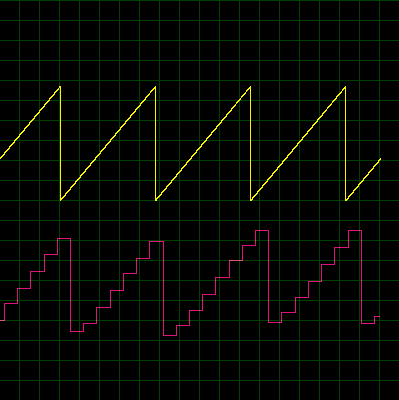
\includegraphics[width=0.5\linewidth]{ImagenesEjercicio1/bit6.png}
\caption{1100 0000}
\end{figure}
\begin{figure}[H]
\centering
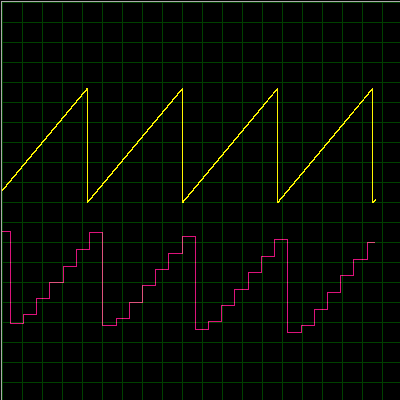
\includegraphics[width=0.5\linewidth]{ImagenesEjercicio1/bit7.png}
\caption{1000 0000}
\end{figure}
\begin{figure}[H]
\centering
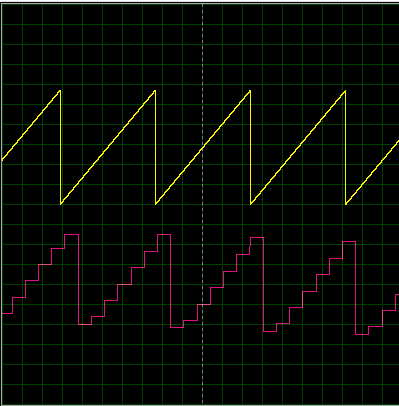
\includegraphics[width=0.5\linewidth]{ImagenesEjercicio1/bit8.png}
\caption{0000 0000}
\end{figure}
\end{multicols}

Se observa que a medida que se sacan bits no solo se pierde la resolución de la señal a la salida del DAC sino que también disminuye la frecuencia de muestreo.

Finalmente, empleando tensiones continuas a la entrada y la funcionalidad de mediciones paso a paso, se completó la siguiente tabla

\begin{table}[H]
\centering
\begin{tabular}{ccc}
\toprule
$Vi \ [mV]$ & $Vadc \ [Binario]$ & $Vo_{DAC} \ [mV]$ \\ \midrule
416.666 & 0001 0101 & 410.01 \\
833.333 & 0010 1011 & 839.84 \\
1250 & 0100 0000 & 1250 \\
1666.66 & 0101 0101 & 1660.15 \\
2083.33 & 0110 1010 & 2070.31 \\
2500 & 1000 0000 & 2500 \\
2916.66 & 1001 0101 & 2910.15 \\
3333.33 & 1010 1010 & 3320.31 \\
3750 & 1011 1110 & 3730.46 \\
4166.66 & 1101 0101 & 4160.15 \\
4583.33 & 1110 1010 & 4570.31 \\
5000 & 1111 1111 & 4980.46 \\ \bottomrule
\end{tabular}
\caption{Tensión a la salida del circuito para entradas dentro de todo el rango.}
\end{table}

Se puede ver que si bien algunos casos poseen un pequeño error, este nunca es mayor a $19.6mV$ excepto para el fondo de escala que se sitúa en $4.98V$ y no $5V$. Para esta cantidad de bits, se obtienen 256 estados posibles, de los cuales $\frac{5V}{256bit} \approx 19.6\frac{mV}{bit}$. Algunos valores no poseen error alguno, esto se debe a que $Vi\cdot \frac{5V}{256bit} \in \mathbb{Q}$

\end{document}